\documentclass[11pt]{article}
\usepackage{techreport}
\title{Did the 2025 US Government Shutdown Change Go-Around Rates?\texorpdfstring{\\}{} A Preregistered Study of Open Flight-Track Data at 76 Airports}
\shorttitle{The 2025 Shutdown and Go-Around Rates}
\author{James Le Cuirot\thanks{Commercial pilot (Senior First Officer), aviation flight safety officer, and aviation safety and compliance consultant specialising in human factors; MSc in Human Factors in Aviation.}\\[2pt] \normalsize CitadelAero}
\date{Working draft v0.1, 12 November 2026}

\begin{document}
\setlength{\emergencystretch}{1.5em}
\maketitle

\begin{abstract}
From 1 October to 12 November 2025 US air traffic controllers worked without pay, and from 7 November the Federal Aviation Administration (FAA) ordered flight reductions at 40 airports, citing unpublished safety data. This preregistered study measured three indicators directly from open flight-track data for 77 days in 2025 and the same weekdays in 2024, at 50 US airports and 26 Canadian and European control airports (about 4.5 million approaches). The primary outcome was the go-around rate. At the US airports it was 4.77 per 1,000 approaches in the 2024 comparison window and 4.64 during the shutdown; at the control airports it was 3.44 and 3.66. The ratio of the US year-on-year change to the control change was 0.93 (95\% interval 0.76 to 1.13). Under the preregistered rules this is inconclusive: no change was detected, a relative rise above about 13\% is excluded on this estimator, but the interval is too wide to declare the absence of a meaningful change. The same comparison for the September before the shutdown, which should have shown nothing, gave 0.78 (0.66 to 0.93), so the two years were not on a common footing before the shutdown began. Correcting for that gave 1.19 (0.91 to 1.53); correcting for weather gave 0.81 (0.68 to 0.95). No estimate shows a clear rise in go-arounds, and the study cannot exclude a moderate one. The share of closely spaced landing pairs and the rate of collision-avoidance resolution advisories both fell at US airports relative to their comparisons, but each measure depends on receiver coverage that changed between the years. The study measures what aircraft did near runways. It does not measure losses of separation, runway incursions or controller workload.
\end{abstract}

\section{Summary of findings}\label{sec:summary}

\begin{enumerate}
\item \textbf{Go-arounds did not detectably change.} During the shutdown window (1 October to 12 November 2025) the 50 US study airports recorded \num{3997} go-arounds in \num{860760} approaches, 4.64 per 1,000. On the same weekdays in 2024 the figures were \num{4062} in \num{851956}, 4.77 per 1,000. The control airports went from 3.44 to 3.66 per 1,000. The preregistered estimate, the ratio of rate ratios, is 0.93 with a 95\% interval of 0.76 to 1.13 (Table~\ref{tab:rates}).
\item \textbf{The preregistered verdict is ``inconclusive''.} The interval includes 1, so no change was detected. It extends below 0.80, so the rule for declaring ``no meaningful change'' is not met. The upper limit excludes a relative increase above about 13\% on this estimator.
\item \textbf{A preregistered check failed, and it weakens the result.} The same comparison in September, before the shutdown, gave 0.78 (0.66 to 0.93). US go-around rates were unusually high in September 2024 (5.40 per 1,000 against 4.26 in September 2025). Measured against that September relationship, the shutdown estimate is 1.19 (0.91 to 1.53). Which reference is right cannot be settled from these data.
\item \textbf{The study was less sensitive than planned.} The preregistration expected to detect a relative change of 21 to 23\%. Day-to-day clustering of go-arounds was stronger than assumed, and the realised figure is about 33\%.
\item \textbf{Individual airports moved in both directions.} Fourteen of the 76 airports show a year-on-year change whose own interval excludes no change, where about four would be expected by chance: seven fell and seven rose. The rises include Boston, Newark, Nashville and Washington Dulles; the falls include New York JFK, Atlanta, San Diego and San Francisco (Figure~\ref{fig:forest}).
\item \textbf{Two secondary indicators fell, with caveats that prevent a firm reading.} The share of landing pairs under 2.5~NM fell at US airports relative to controls (0.81; interval 0.73 to 0.90 when days are resampled, 0.55 to 1.22 when airports are resampled). Resolution advisories recorded near US airports fell relative to 2024 (0.73; 0.63 to 0.85). Both measures depend on how much of the traffic the receiver network saw, and that changed between the years.
\end{enumerate}

The rest of the paper gives the background, the method as preregistered, the results in full, and a closing section on what the study does and does not show.

\section{Background}\label{sec:background}

A lapse in appropriations began on 1 October 2025 and ended on 12 November 2025. The FAA's emergency order of 7 November states that ``air traffic controllers have been working without pay since October 3, 2025''~\cite{faa2025order1}. The same order required airlines to cut scheduled domestic flights at 40 ``High Impact Airports'', by 4\% from 7 November rising to 10\% by 14 November. It also allowed air traffic control at short-staffed facilities to withhold services to aircraft flying under visual flight rules, including traffic-pattern operations and practice approaches~\cite{faa2025order1}. A replacement order effective 13 November held the reduction at 6\% and prohibited most general aviation at 12 of the airports~\cite{faa2025order2}. The orders were cancelled with effect from 6:00~a.m. Eastern time on 17 November~\cite{faa2025cancel}.

The first order justified the reductions by reference to safety data: the FAA had ``assessed voluntary safety reports submitted for the month of October'' and observed ``evidence of increased stress on the NAS in aviation safety data'', the NAS being the national airspace system~\cite{faa2025order1}. The cancellation notice says that these data ``indicated a correlation between ATO staffing and stress on the NAS''~\cite{faa2025cancel}. None of the three notices gives a number. A Congressional Research Service review published in October 2026 reports delay and cancellation counts for the shutdown but no safety-event data and cites no empirical safety study~\cite{crs2026}.

Published measurements of the shutdown concern delay and disruption. The Federal Reserve Bank of Richmond compared delays at 82 airports inside and outside the shutdown window and found statistically significant increases at six: Boston, Washington National, Newark, New York JFK, LaGuardia and San Francisco~\cite{wong2025}. A student report examined cancellations at Orlando~\cite{cruz2025}. Searches on 11 and 12 November 2026 found no study that measured a safety indicator for this period from flight data. The searches did not cover every index (Section~\ref{sec:limits}).

Go-arounds can be detected in crowd-sourced surveillance data. Published rates from such data are a few per 1,000 approaches: about 2.5 per 1,000 at Mumbai~\cite{proud2020}, ``one to three per 1000 commercial flight approaches'' as a general figure quoted in a study of San Francisco~\cite{kumar2021}, and 1.5 to 6 per 1,000 across 20 large European airports~\cite{figuet2023}. A go-around is a normal, safe manoeuvre. Its rate is used here as an indicator of how often an approach could not be completed, for whatever reason: spacing, an occupied runway, an unstable approach, weather or an instruction from the tower.

The direction of any shutdown effect was not obvious in advance. Controllers under strain might space aircraft less accurately, which would raise go-arounds. Short-staffed facilities also reduce arrival rates and add spacing, which would lower them. The preregistration stated that a flat result was the most likely outcome and would be reported as such.

\section{Method}\label{sec:method}

The hypotheses, airports, windows, measures, exclusions, analysis and decision rules were fixed in a preregistration committed to a public repository on 11 November 2026, before any study-window data had been downloaded (\code{PREREGISTRATION.md}, commit \code{bfb0eae}). The time-stamp is that of the public commit; the document was not lodged with a registry. Section~\ref{sec:deviations} lists every departure from it.

\subsection{Data}

Flight tracks came from the adsb.lol archive, which publishes one file set per day of all aircraft traces received by its volunteer network~\cite{adsblol}. Seventy-seven days were processed for 2025 (1 September to 16 November) and 77 for 2024 (2 September to 17 November). Each 2024 day is the 2025 date minus 364 days, so the two years are aligned by day of the week. Every download was checked against the archive's published size. Runway positions came from OurAirports~\cite{ourairports}. Hourly weather reports (METAR) for every study airport came from the Iowa Environmental Mesonet~\cite{iem}.

Only aircraft whose type code is in fixed lists of airline jets and business jets were kept, and only positions within 15~NM of a study airport and below \num{7000}~ft above it.

\subsection{Airports}

Eighty-four airports were preregistered: the 40 airports of the FAA order, 15 other US airports, 4 Canadian and 25 European. A coverage rule fixed in advance removed any airport that, in either year, had fewer than 60 of 77 days with at least 30 detected approaches. It removed eight: Houston Intercontinental, Columbus, Jacksonville, Kansas City, Pittsburgh, Vancouver, Oslo and Paris Orly. The analysis therefore covers 39 order airports, 11 other US airports, 3 Canadian and 23 European airports.

\subsection{Measures}

\paragraph{Go-around rate (primary).} A landing is the last airborne position of a flight on short final to a runway (within 150~m of the centreline, below 700~ft, track within 15 degrees of the runway) after a descent of at least \num{1500}~ft. A go-around is a local altitude minimum below \num{3000}~ft above the airport, aligned with a runway, preceded by a descent of at least 800~ft and followed by a climb of at least 500~ft with no ground contact. The rate is go-arounds divided by landings plus go-arounds. The detection code was carried over unchanged from an earlier study by the author and was not tuned on these data.

\paragraph{Tight-pair share.} For each pair of consecutive landings on the same runway within 400 seconds, the follower's distance from the threshold was taken at the moment the leader was last seen airborne. The measure is the share of pairs in which that distance was under 2.5~NM.

\paragraph{Resolution advisory rate.} The archive records the resolution advisory (RA) messages that aircraft collision-avoidance systems (TCAS) broadcast. An event is the first such message from an aircraft after at least two minutes without one, within 15~NM of a US study airport and below \num{7000}~ft above it. The rate is events per 1,000 detected approaches. Pilot days showed almost no RA messages near the European airports, so this analysis has no control group. Such messages are only received when the aircraft is interrogated within range of a receiver~\cite{schafer2019}, so capture is partial.

\paragraph{Exclusions.} An aircraft that made three or more go-arounds at one airport in one day was treated as training, test or flight-inspection activity and all its approaches there that day were removed (216 approaches, including 177 go-arounds), as were 64 approaches by FAA flight-inspection callsigns.

\subsection{Design and analysis}

The primary estimate is a ratio of rate ratios: the US go-around rate in the shutdown window divided by the US rate on the same weekdays in 2024, divided by the same quantity for the control airports. It was estimated by Poisson regression with a fixed effect for each airport. A value of 1 means US airports changed between the years exactly as the control airports did. Intervals come from resampling whole days \num{2000} times, keeping each 2025 day with its 2024 partner, because weather makes go-arounds cluster by day. A second interval resamples airports.

The decision rules were fixed in advance. A change is detected if the 95\% interval excludes 1. No meaningful change is declared if the interval lies wholly inside 0.80 to 1.25. Anything else is inconclusive.

Preregistered secondary analyses were: the same estimate for September (a placebo, since the shutdown had not begun); the shutdown estimate divided by the September estimate (``baseline-adjusted''); separate estimates for 1 October to 6 November (phase A, before the flight reductions), 7 to 16 November (phase B) and 31 October to 9 November (the period of most reported staffing shortfalls); order airports and other US airports separately; each control region alone; airline jets only; and the estimate without the training-flight exclusion. A weather-adjusted model added three airport-day covariates: the share of hours with a ceiling under \num{1000}~ft or visibility under 3 statute miles, whether any gust reached 25~kt, and whether a thunderstorm was reported.

\subsection{Blinding}

The processing code was built and tested on three days outside the study window. While the 154 study days were processed, only counts of approaches were displayed. The analysis script was committed before use and was run once on the complete data.

\subsection{Departures from the preregistration}\label{sec:deviations}

\begin{enumerate}
\item The weather data were obtained after registration but before any outcome was computed. The covariate definitions and the model were added to the preregistration as a dated addendum at that point (commit \code{946239f}).
\item The preregistration said the median follower distance would be reported with the spacing result. The analysis script omitted it. It was computed after the results were known, by a script that applies the registered definition.
\item Four analyses were added after the results were known and are labelled exploratory wherever they appear: a weather-adjusted September placebo; a model adjusted for both September and weather; the RA ratio by phase; and year-on-year traffic counts by phase.
\item Six days failed during processing when the workspace ran out of memory. All six completed on retry and none was dropped.
\end{enumerate}

\section{Results}\label{sec:results}

\subsection{Go-arounds}

\begin{table}[t]
\centering
\caption{Go-arounds and approaches by group, year and window. Rates are per 1,000 approaches. The 2024 windows are the same weekdays, 364 days earlier. \source{\code{results/results.json}}}\label{tab:rates}
\begin{tabular}{llrrr}
\toprule
Window & Group and year & Go-arounds & Approaches & Rate \\
\midrule
Shutdown & US 2024 & \num{4062} & \num{851956} & 4.77 \\
(1 Oct--12 Nov) & US 2025 & \num{3997} & \num{860760} & 4.64 \\
 & Control 2024 & \num{1273} & \num{369735} & 3.44 \\
 & Control 2025 & \num{1423} & \num{388701} & 3.66 \\
\midrule
September & US 2024 & \num{3127} & \num{579406} & 5.40 \\
(1--30 Sep) & US 2025 & \num{2504} & \num{587234} & 4.26 \\
 & Control 2024 & \num{908} & \num{260965} & 3.48 \\
 & Control 2025 & \num{982} & \num{281238} & 3.49 \\
\bottomrule
\end{tabular}
\end{table}

In the shutdown window the US rate fell by 0.12 per 1,000 between the years and the control rate rose by 0.22, a difference of $-0.34$ per 1,000 (Table~\ref{tab:rates}). The ratio of rate ratios is 0.93. The day-resampled interval is 0.76 to 1.13 and the airport-resampled interval is 0.82 to 1.05. Neither excludes 1.

\begin{table}[t]
\centering
\caption{Estimates of the ratio of rate ratios for go-arounds, with 95\% intervals from resampling days. Values below 1 mean US go-arounds fell relative to the control airports. Rows marked E are exploratory. \source{\code{results/results.json}, \code{results/supplementary.json}}}\label{tab:estimates}
\begin{tabular}{lrl}
\toprule
Analysis & Estimate & 95\% interval \\
\midrule
Primary: shutdown window, all airports & 0.93 & 0.76 to 1.13 \\
September placebo & 0.78 & 0.66 to 0.93 \\
Shutdown, adjusted for September & 1.19 & 0.91 to 1.53 \\
Shutdown, adjusted for weather & 0.81 & 0.68 to 0.95 \\
September placebo, adjusted for weather (E) & 0.77 & 0.65 to 0.90 \\
Shutdown, adjusted for September and weather (E) & 1.07 & 0.84 to 1.38 \\
\midrule
Phase A, 1 October to 6 November & 0.91 & 0.73 to 1.13 \\
Phase B, 7 to 16 November & 0.90 & 0.65 to 1.21 \\
Peak staffing shortfalls, 31 October to 9 November & 1.07 & 0.92 to 1.26 \\
\midrule
FAA-order airports only & 0.92 & 0.75 to 1.11 \\
Other US airports only & 1.03 & 0.80 to 1.36 \\
Europe as the only control & 0.92 & 0.75 to 1.13 \\
Canada as the only control & 1.00 & 0.72 to 1.32 \\
Airline jets only & 0.93 & 0.76 to 1.13 \\
Without the training-flight exclusion & 0.94 & 0.77 to 1.14 \\
\bottomrule
\end{tabular}
\end{table}

\begin{figure}[t]
\centering
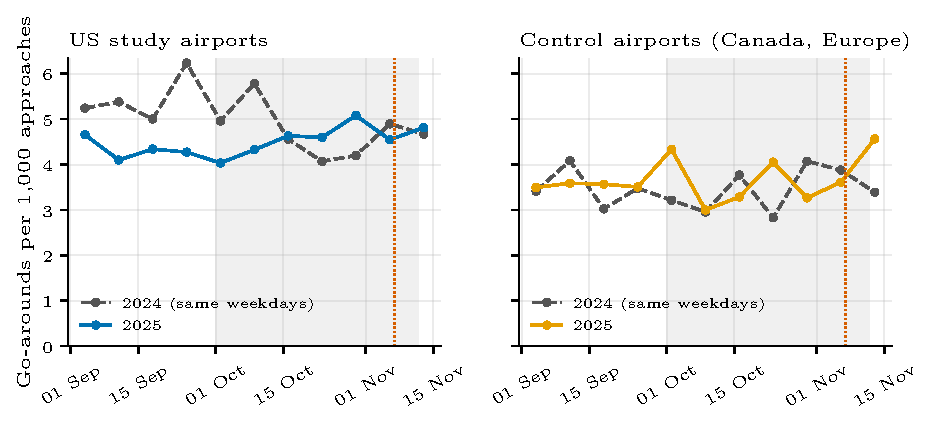
\includegraphics[width=\linewidth]{figures/fig_weekly_goaround.pdf}
\caption{Weekly go-around rate. Solid lines are 2025; dashed lines are the same weekdays in 2024. The shaded band is the shutdown; the dotted line marks the start of the flight reductions on 7 November.}\label{fig:weekly}
\end{figure}

\paragraph{The September placebo.} The September estimate is 0.78 (0.66 to 0.93). A sound comparison would have given a value near 1 there. Figure~\ref{fig:weekly} shows why it did not: US rates in September and early October 2024 ran at 5 to 6 per 1,000, well above the same weeks of 2025, while the control airports were level. Weather as measured here does not explain the gap. With the three weather covariates the September estimate is 0.77 (exploratory). The cause was not identified. Candidates that this study could not test include convective weather that hourly airport reports capture poorly, runway works, and changes in which aircraft the receiver network saw.

\paragraph{What the placebo does to the main result.} If the September relationship is taken as the baseline, the shutdown estimate is 1.19 (0.91 to 1.53): US go-arounds rose relative to their own September by more than the control airports did. Within 2025 the US rate went from 4.26 per 1,000 in September to 4.64 in the shutdown window, a rise of 9\%, while the control rate rose 5\%. Within 2024 the US rate fell 12\% over the same weeks. The baseline-adjusted figure therefore rests on the assumption that 2025 would have repeated the 2024 autumn decline. If September 2024 was the unusual month, the primary estimate is the better guide; if the September gap reflects a lasting difference between the years, the baseline-adjusted estimate is. The two bracket the answer, and both intervals include 1.

\paragraph{Weather.} Low cloud or visibility was the strongest of the three covariates: an airport-day wholly below the threshold had 3.6 times the go-around rate of a day wholly above it; gusts of 25~kt or more multiplied the rate by 1.4, and a reported thunderstorm by 1.4. Adjusting for them moves the shutdown estimate from 0.93 to 0.81 (0.68 to 0.95). The movement comes mainly from the control airports, which had low cloud or visibility in 20\% of hours in the 2024 window and 12\% in 2025, yet recorded more go-arounds in 2025. On the preregistered rule this interval excludes 1. It is not treated as a finding that go-arounds fell, for three reasons: the analysis is secondary; the September placebo still fails after the same adjustment; and with both adjustments together the estimate is 1.07 (0.84 to 1.38).

\paragraph{Phases, groups and exclusions.} No phase, airport group or exclusion variant gives an interval that excludes 1 (Table~\ref{tab:estimates}). The estimate for the ten days of most reported staffing shortfalls is 1.07 (0.92 to 1.26). In phase B the order airports did not differ detectably from the other US airports (0.85; 0.60 to 1.18). Leaving out any single airport moves the primary estimate only between 0.91 and 0.95. Approaches at the order airports were 0.5\% higher than in 2024 in phase A and 3.7\% lower in phase B (exploratory), so the ordered reductions are visible in the data but small.

\paragraph{Sensitivity achieved.} The standard error of the log estimate was 0.102, against 0.044 if go-arounds were independent events. The realised detectable relative change, on the preregistered definition, is 33\%.

\subsection{Variation between airports}

\begin{figure}[p]
\centering
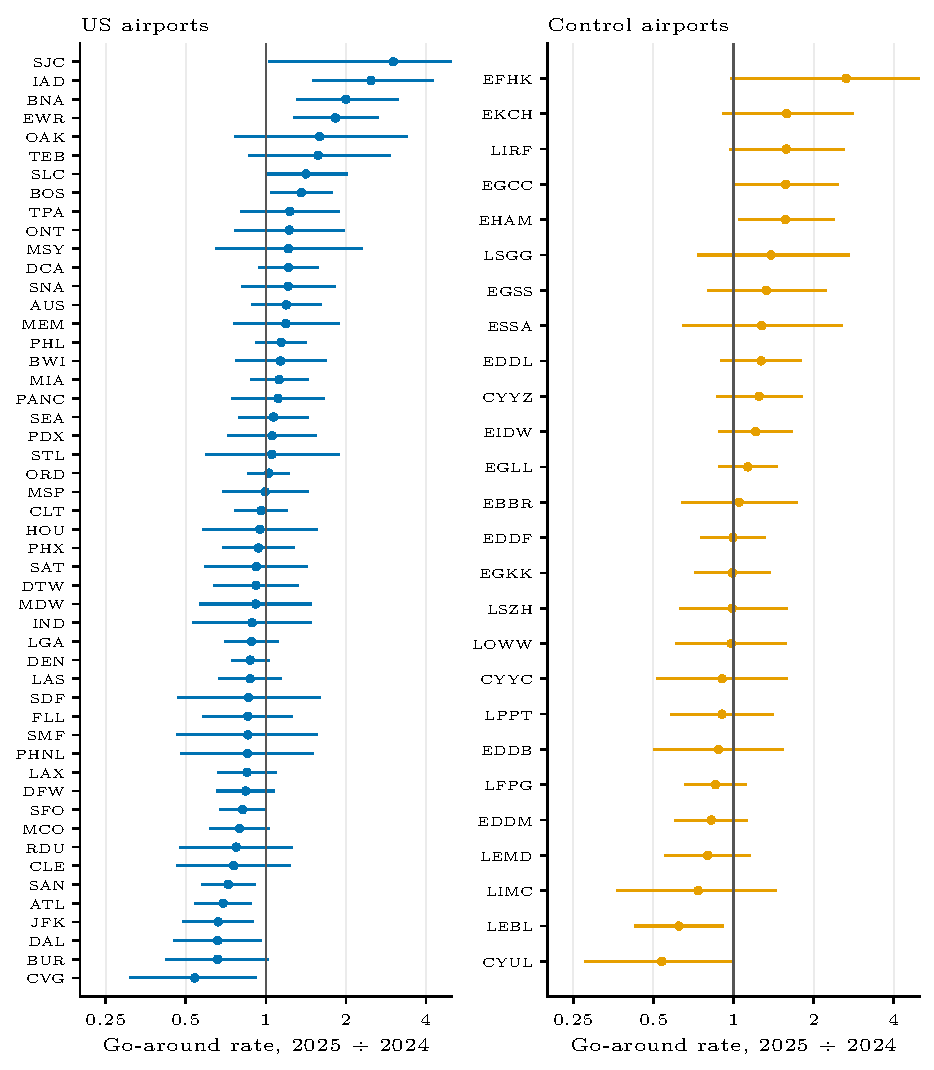
\includegraphics[width=0.95\linewidth]{figures/fig_airport_forest.pdf}
\caption{Year-on-year go-around rate ratio in the shutdown window for each airport, with exact 95\% intervals. These are single-airport comparisons of 2025 with 2024 and include no control group.}\label{fig:forest}
\end{figure}

Airports differed from one another by more than chance alone would produce (Figure~\ref{fig:forest}). Among the 50 US airports the between-airport standard deviation of the log rate ratio was 0.20, so a typical airport's year-on-year change differed from the average by about a fifth in either direction; among the control airports it was 0.18. Eleven US airports have intervals that exclude 1. Five rose: Boston (1.36), Newark (1.83), Nashville (2.00), Washington Dulles (2.48) and San Jose (3.0, from 5 and 14 events). Six fell: New York JFK (0.66), Atlanta (0.69), San Diego (0.72), San Francisco (0.82), Cincinnati (0.54) and Dallas Love Field (0.66). Three control airports also moved: Amsterdam (1.57) and Manchester (1.57) rose and Barcelona fell (0.62).

These single-airport figures need care. They have no control group, so local weather, runway works and procedure changes are all mixed in. Detected approaches at Nashville rose by 60\% between the years and at Zurich more than doubled, which points to a change in receiver coverage at those airports and makes their rates hard to compare across years. Of the six airports where the Richmond study found significant delay increases~\cite{wong2025}, the go-around rate rose at Boston and Newark, rose within its interval at Washington National (1.21), and fell at JFK, San Francisco and LaGuardia (0.88). Delay during the shutdown was not a guide to the go-around rate.

\subsection{Spacing on final}

\begin{figure}[t]
\centering
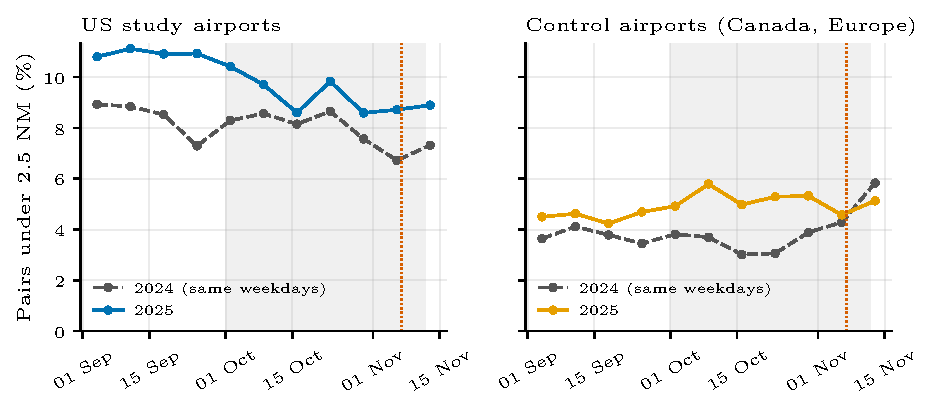
\includegraphics[width=\linewidth]{figures/fig_weekly_spacing.pdf}
\caption{Weekly share of same-runway landing pairs in which the follower was within 2.5~NM of the threshold when the leader was last seen airborne.}\label{fig:spacing}
\end{figure}

The share of tight pairs rose between the years in both groups: from 7.9\% to 9.2\% at US airports and from 3.7\% to 5.1\% at control airports. The ratio of rate ratios is 0.81. Resampling days gives 0.73 to 0.90; resampling airports gives 0.55 to 1.22. The September placebo is 1.03 (0.94 to 1.14), and the baseline-adjusted estimate, which the preregistration named as the main spacing result, is 0.78 (0.68 to 0.90; adjusted $p=0.001$). The median follower distance at US airports was 4.32~NM in the 2024 window and 4.22~NM in the shutdown window; at control airports 5.00 and 4.75~NM.

Figure~\ref{fig:spacing} shows the pattern behind the estimate. The US tight-pair share ran near 11\% through September 2025 and dropped to between 8.6\% and 9.8\% from the second week of October. That is consistent with slightly wider spacing on final at US airports during the shutdown. Three things prevent a firm conclusion. The rise between the years in both groups is what more complete receiver coverage would produce, because a pair can only be measured when both aircraft are seen, and coverage did not grow equally everywhere. The US share also declined through the autumn of 2024. And the airport-resampled interval includes 1: the median US airport showed no change in its tight-pair share (ratio 0.99; exploratory), so the pooled result is carried by a subset of airports.

\subsection{Resolution advisories}

\begin{figure}[t]
\centering
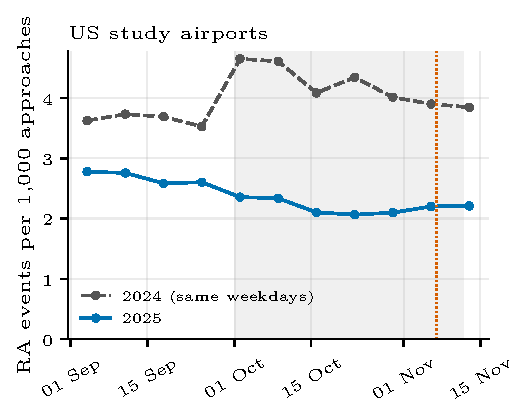
\includegraphics[width=0.58\linewidth]{figures/fig_weekly_ra.pdf}
\caption{Weekly resolution advisory events per 1,000 detected approaches near US study airports.}\label{fig:ra}
\end{figure}

RA events near US study airports numbered \num{2138} in September 2024 (3.69 per 1,000 approaches) and \num{3616} in the 2024 comparison window (4.24); \num{1534} in September 2025 (2.61) and \num{1883} in the shutdown window (2.19). The preregistered ratio is 0.73 (0.63 to 0.85; adjusted $p<0.001$): the rate fell from September into the shutdown in 2025 and rose over the same weeks in 2024. Excluding Washington National and Burbank, where procedures changed during 2025, gives 0.76 (0.66 to 0.89). The ratio was already 0.74 (0.63 to 0.86) in phase A, before the general aviation restrictions (exploratory).

The preregistration classed this analysis as descriptive support, and it should be read that way. The rate was about 30\% lower in 2025 than in 2024 even in September, before the shutdown, which shows that something other than the shutdown separates the two years: procedure changes after the January 2025 collision at Washington, changes in the receiver network, or changes in how the archive decodes these messages. Figure~\ref{fig:ra} shows a step up in early October 2024 and a gradual decline through autumn 2025. A plausible operational reading of the decline is that less visual-flight-rules traffic was flying near these airports, or receiving service, during the shutdown. This study has no data on that traffic and cannot test it.

\section{Limitations}\label{sec:limits}

\begin{itemize}
\item \textbf{The comparison years were not equivalent before the shutdown.} The failed September placebo is the main limitation. It means the control airports did not remove everything that differed between the years, and the primary estimate could be biased in either direction.
\item \textbf{Sensitivity.} The study could detect a relative change of about a third. A rise of 10 or 20\% in go-arounds, if it happened, would not have been detected reliably.
\item \textbf{Receiver coverage changed.} The 2025 archive is about 45\% larger than the 2024 archive. Approach counts at most study airports were stable, but at some they rose sharply. Go-around detection needs continuous low-altitude data, so better coverage could raise the detected rate at an airport without any change in flying.
\item \textbf{Go-around detection was not validated against a reference for these airports.} The rules were carried over from an earlier study. Published work finds that detection from crowd-sourced data tends to miss go-arounds~\cite{monstein2022}. A constant miss rate would cancel in the ratios; a miss rate that changed with coverage would not.
\item \textbf{The control airports are on other continents.} Autumn weather in Europe and Canada is not the weather of the United States. Whether European or Canadian air traffic services had disruptions of their own in the window was not checked.
\item \textbf{The reason for each go-around is unknown.} The data cannot separate a go-around ordered for spacing from one flown for wind shear or an unstable approach.
\item \textbf{The shutdown window mixes several things.} From 7 November the flight reductions, the general aviation restrictions and the withdrawal of some services to visual-flight-rules traffic all changed the traffic itself. Other events in the window include the UPS accident at Louisville on 4 November 2025 and, in the 2024 comparison period, two major hurricanes in the south-eastern United States.
\item \textbf{Staffing was not measured.} The study compares periods, not facilities with and without shortfalls. A facility-level analysis using the FAA's staffing notices was considered and not preregistered, because the notices could not be retrieved.
\item \textbf{The literature search was not exhaustive.} Google Scholar, SSRN and conference proceedings were searched by keyword, not systematically.
\item \textbf{The preregistration is time-stamped only by a public repository commit.}
\end{itemize}

\section{What the study does and does not show}\label{sec:closing}

\paragraph{It shows} that, across 50 US airports and about 860,000 approaches during the shutdown, the rate at which jets abandoned approaches was close to the rate a year earlier, and that no version of the analysis found a clear increase. The primary estimate excludes a rise of more than about 13\% relative to the control airports. It also shows large differences between airports, in both directions, that were unrelated to where delays were worst.

\paragraph{It does not show} that the shutdown had no effect on safety. The formal result is inconclusive. The check designed to confirm that the comparison was fair failed. A moderate rise in go-arounds cannot be excluded once that failure is allowed for, and neither can a fall. The study did not measure the events the FAA cited, which were voluntary reports and unspecified safety data, and it did not measure losses of separation, runway incursions, communication errors or controller fatigue. A go-around rate that holds steady is compatible with a system under strain that is protecting its margins by slowing down, and the spacing result, for what it is worth, points that way.

\paragraph{What would settle it.} Three things would sharpen the answer: the FAA's own counts of the events it referred to; a facility-level comparison that uses the dates and places of staffing shortfalls; and a third comparison year, which would show whether autumn 2024 or autumn 2025 was the unusual one.

\section*{Acknowledgement}
\paragraph{AI assistance.} Literature searches, drafting and source verification were carried out with AI assistance (Claude, Anthropic) under the author's direction, as were the data processing code and analysis. An independent AI-assisted audit checked the analysis and the operational interpretation, and its findings were addressed before this version. The author is responsible for the final text.
\paragraph{Competing interests.} The author is the founder of CitadelAero, which builds AI tools for aviation.
\paragraph{Disclaimer.} The views expressed are the author's own and do not represent those of any employer or regulator. Nothing here is operational, legal or regulatory advice.
\paragraph{Materials.} The preregistration, code, airport-day data, results, verification log and audit record for this paper are at \url{https://github.com/JamesLeCuirot/Research/tree/main/papers/08-shutdown-safety-indicators}.

\bibliographystyle{IEEEtran}
\bibliography{references}
\end{document}
